\chapter{Actors}
\label{ch:actors}

Actors specify a role played by a user or a system for the purposes of a clearer definition.
In this chapter, we will outline the actors in our system.
For a graphical representation of the actors and their interactions, please see figure~\ref{fig:bigpicture}.

\section{Big Picture}\label{sec:big-picture}

\begin{figure}[H]
	\begin{center}
		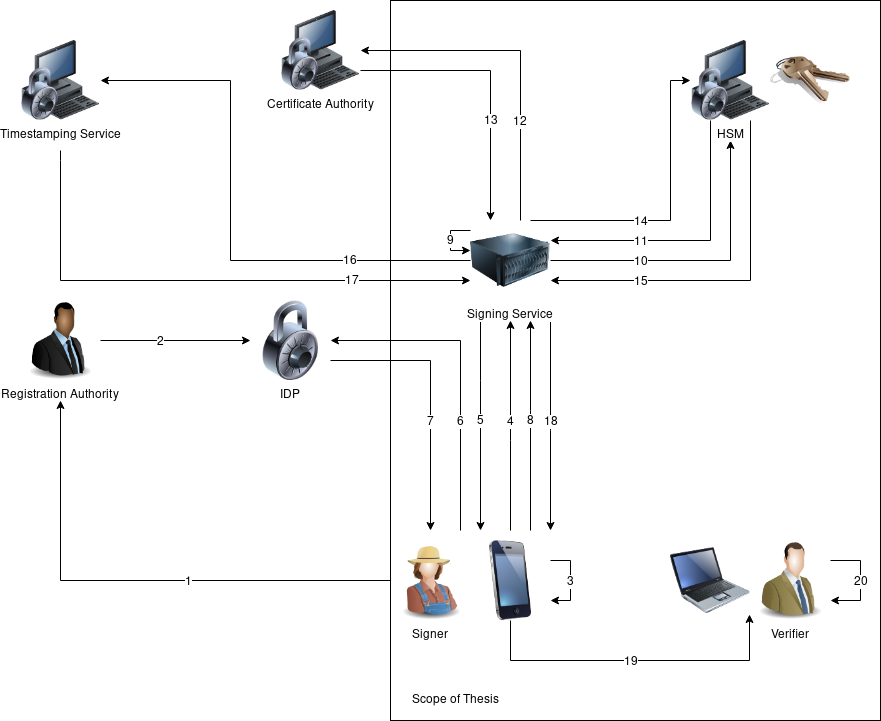
\includegraphics[scale=0.55]{images/BigPicture.png}
		\caption{The Actors in our system, and the scope of our thesis}
		\label{fig:bigpicture}
	\end{center}
\end{figure}

The following subsections provide a description of the interactions as numbered in figure~\ref{fig:bigpicture}.

\subsection{Registration}\label{subsec:registration}
\begin{enumerate}
    \item Registration of identity with the \gls{RA} (Authenticator)

    A pre-requisite for using our signing service is that the user (Verifier) is registered with an \gls{IDP} trusted by the Signing Service.
    The user registers at the \gls{RA} by proving their identity to it.
    In most cases, this process needs to be completed only once per user.

    \item Propagate identity to \gls{IDP} (Identifier)

    After the identity has been confirmed, the \gls{RA} propagates this fact to the \gls{IDP}.
    From this point on the user is known to the \gls{IDP} and the user may authenticate themselves to third parties with it.
    (The \gls{RA} and the \gls{IDP} may be the same entity.)

\end{enumerate}

\subsection{Identification}\label{subsec:identification}
\begin{enumerate}[resume]
    \item Generate document hash

    The user (Verifier) generates the hashes of the document(s) they wish to sign.
    This is needed before the identification step in order to prevent signing of arbitrary documents by securely binding the document hashes to the authentication request and subsequent identity assertion,
    as we've shown in our previous work~\cite{projekt2}.

    \item Send hash to signing service

    The user sends the hashes of the documents they generated in the previous step to the signing service.

    \item Receive \gls{OIDC} redirect to \gls{IDP}

    The signing service constructs \gls{OIDC} redirects for all configured \gls{IDP}s,
    and returns them to the user.
    These redirects contain a strong cryptographic link to the hashes submitted in the previous step.

    \item Login to \gls{IDP}

    The user follows the redirect they received in the previous step and authenticates with the \gls{IDP} in order for it to confirm their identity.

    \item Receive ID token

    After successful authentication, the user receives an authentication token from the \gls{IDP},
    signed by the \gls{IDP}, as proof of their identity.

    \item Send ID token to signing service

    The user sends the ID token from the previous step to the signing service.

    \item Verify ID token

    The signing service validates the ID token (\gls{JWT}) and checks its contents,
    in order to confirm whether the secure linking of the user's intent to sign specific documents with the authentication is valid.
\end{enumerate}


\subsection{Signature Generation}\label{subsec:signature-generation}
\begin{enumerate}[resume]
    \item Request signing key \gls{CSR} from \gls{HSM}

    The signing service requests the \gls{HSM} to generate a new signing key in the name of the user.

    \item Receive \gls{CSR}

    The \gls{HSM} generates this new signing key and returns the \acrfull{CSR}.

    \item Send \gls{CSR} to \gls{CA}

    The signing service sends the \gls{CSR} to the \gls{CA}.

    \item Receive signed certificate

    The \gls{CA} signs the \gls{CSR} and returns the signed certificate to the signing service.

    \item Request signature from \gls{HSM}

    The signing service sends the data to be signed, which includes the document hashes, to the \gls{HSM}.

    \item Receive signature

    The \gls{HSM} signs the data, using the signing key generated in step 10, and returns the signature to the signing service.

    \item Request timestamp from \gls{TSS}

    The signing service sends the hash value of the signature data to the \gls{TSS}.

    \item Receive timestamp

    The \gls{TSS} adds a timestamp to the signature and signs it,
    and returns the timestamp along with its signature to the signing service.

    \item Send signature to signer

    The signing service constructs the final signature file containing at least the signed hash,
    the signed timestamp, the ID token and the chains of all used certificates as well as revocation information to the user.
\end{enumerate}

Steps 16 and 17 correspond exactly to \gls{RFC} 3161~\cite{rfc3161}.

\subsection{Signature Verification}\label{subsec:signature-verification}
\begin{enumerate}[resume]
    \item Send document and signature to receiver (Verifier)

    The user sends the document and the signature to the intended receiver.

    \item Verify document and signature

    The receiver uses the validation tool to validate the document and signature.
\end{enumerate}

\section{The Signer}
\label{sec:actorsigner}
The Signer is the person who wishes to have the signing server sign one or more documents in their name.
For example, a medical professional issuing a prescription for medication to a patient.

\section{The Verifier}
\label{sec:actorverifier}
The Verifier is the person who wishes to verify the integrity of a document and its signature.
For example, the pharmacist whom the patient gives the prescription to (as previously signed by The Signer as specified in section~\ref{sec:actorsigner}) in order to purchase the medication prescribed by the medical professional.

\section{The Authenticator}
\label{sec:actorauthenticator}
The Authenticator is the system who authenticates The Signer as specified in section~\ref{sec:actorsigner}.
In \gls{NIST} terminology~\cite{nistdigitalidentityguidelines}, this is the entity establishing the \gls{IAL}.
In order for The Authenticator to be able to authenticate The Signer,
they must have been registered with The Authenticator by The Identifier as specified in section~\ref{sec:authoridentifier}.

\section{The Identifier}
\label{sec:authoridentifier}
The Identifier is the system or person who asserts the identity of The Signer.
In order for the signing service to issue qualified signatures as defined by Swiss Federal Assembly legislation~\cite{zertes} and Swiss Federal Council regulations~\cite{vzertes},
the identity must be proven in-person using a government-issued photographic identification document such as a passport.

\section{The Signing Service}
\label{sec:actorsigningservice}
The Signing Service is the system who actually creates the signatures on behalf of the user.
It generates the signing keys and requests the \gls{CA} (actor~\ref{sec:actorca}) to sign them.

\section{The Certificate Authority}
\label{sec:actorca}
The \gls{CA} is the system who signs the signing keys generated by the Signing Service (actor~\ref{sec:actorsigningservice}).
The \gls{CA} offers \gls{CRL} and \gls{OCSP} responders.
